\section{Normalization of $\lambda$-terms is a first-order transduction}
\label{sec:eval}

\newcommand{\lambdaterm}{$\lambda$-term }
\newcommand{\lambdaterms}{$\lambda$-terms }

\newcommand{\NonLinTerms}[2]{\Lambda_{#1} #2}
\newcommand{\LinTerms}[2]{\mathsf{Lin}_{#1} #2}

 \newcommand{\rlambda}{\ranked{\Lambda}}
 \newcommand{\rlambdalin}{\ranked{\Lambda^{\sf{lin}}}}
 \newcommand{\rlambdathin}{\ranked{\Lambda^{\sf{thin}}}}


\newcommand{\thinterm}[1]{\ranked{\mathsf{Thin}_{#1}}}

In this part of the appendix, we show Theorem~\ref{thm:normalise}, which says that under some restrictions, evaluation of $\lambda$-terms is a first-order transduction. Before proving this result in~\ref{sec:evaluation-lambda}, we will first explain in~\ref{sec:explaining-restrictions} why these restrictions are unavoidable. Then we show in \ref{sec:restrictions-are-fo} that the set of $\lambda$-terms satisfying these restrictions form a first-order tree language. This result will be useful for the proof of Theorem~\ref{thm:normalise}.



\subsection{Explaining the restrictions}\label{sec:explaining-restrictions}

Recall that Theorem~\ref{thm:normalise} says that evaluation of $\lambda$-terms is derivable under two assumptions:
the input term should be linear (actually it could be also affine),  and it could be typed using a fixed finite set of types. 

If the linearity condition is removed, and because of iterated duplication, the normal form of a well-typed $\lambda$-term can be exponential (or worse, see~\cite[Section 3.6]{sorensen_lectures_2006}), as shown by the following example.
 
\begin{example}\label{ex:exponential}
    Assume that we have two variables $\typevar x  \otype$ and $\typevar y {\otype \to \otype \to \otype}$ and consider the $\lambda$-terms defined by:
    \begin{align*}
        M_0 \eqdef \typevar x \otype \qquad M_{n+1} = (\lambda \typevar x  \otype . \typevar y {\otype \to \otype \to \otype}  \typevar x  \otype \typevar x  \otype)M_n.
    \end{align*}
    The $\lambda$-term $M_n$ is well-typed and of type $\otype$. It has size linear in $n$, but its normal form has size at least $2^n$. 
    % as shown in the following picture, which uses variables $x : \otype$ and  $z : \otype \to \otype \to \otype$.
    % \mypic{44}
\end{example}
If there was a first-order transduction normalizing these terms, it would be exponential-size increase, which is not possible since all first-order transductions are linear-size increase. 
% For this reason, we  limit attention to linear  $\lambda$-terms.
%: a $\lambda$-term is called \emph{affine} if every bound variable is used at most once in its scope, but free variables are allowed to appear multiple times.  For example, 
%\begin{align*}
%\typevar z {\otype \to \otype \to \otype} \big(\lambda \typevar x \otype.  \typevar y {\otype \to \otype} (\typevar y {\otype \to \otype}  \typevar x \otype)\big) \big(\lambda \typevar x \otype.  \typevar y {\otype \to \otype} (\typevar y {\otype \to \otype}  \typevar x \otype)\big)
%\end{align*}
%is affine, even if $\typevar y {\otype \to \otype}$ appears four times. If we prepend $\lambda \typevar y {\otype \to \otype}$, then the $\lambda$-term ceases to be affine.

Being linear alone is not enough to normalise terms with first-order transductions. Another obstacle is terms that use types of unbounded complexity, as illustrated in the following example. 

\begin{example}\label{ex:affine-not-enough}
Consider the following $\lambda$-terms, which have types of 
unbounded size: 
\begin{align*}
M_n = \overbrace{\lambda \typevar x \otype. \lambda \typevar  x \otype. \cdots \lambda \typevar  x \otype.}^{\text{$n$ times}} \typevar  x \otype
\end{align*}
This is a well-typed affine term, whose type is 
\begin{align*}
\otype^n \to \otype \qquad \eqdef \qquad  \overbrace{\otype \to \otype \to \cdots \to \otype}^{\text{$n+1$ arrows}}
\end{align*}
    To $M_n$, apply  $m$ arguments of type $\otype$:
    \begin{align}\label{eq:complicated-term}
    M_n \overbrace{\typevar y \otype \ \typevar y {\otype} \cdots \typevar y{\otype} }^{\text{$m$ times}}.
    \end{align}
    We claim that the above $\lambda$-term cannot be normalised using a first-order transduction, or even a monadic second-order transduction. In order to normalise, a transduction would need to be able to compare the numbers $n$ and $m$ as follows:  if $m < n$  the normal form contains $\lambda$, if $m=n$  the normal form does not contain $\lambda$, and if $m > n$ then the normal form is undefined because the $\lambda$-term is not well-typed.  Whether or not a $\lambda$-term (seen as a tree over a finite alphabet) contains $\lambda$ is a first-order definable property, and first-order definable properties are preserved under inverse images of first-order transductions. Therefore, if normalisation would be a first-order transduction,
then there would be a first-order formula which would be true for terms of the form~\eqref{eq:complicated-term} with $m>n$ and which would be false for terms of the form~\eqref{eq:complicated-term} with $m=n$. Such a formula cannot exist, which can be shown using a pumping argument or Ehrenfeucht-Fra\"iss\'e games. 
\end{example}

\subsection{Well-typedeness} \label{sec:restrictions-are-fo}
In general, well-typedeness is not a FO property (actually not even a MSO property) as shown by Example~\ref{ex:exponential} in Section~\ref{sec:one-register}.
However, checking whether the type of a \lambdaterm and the type of its sub-terms all belong to a fixed finite set of types if a FO property. 
%Note that contrarily to normalization, well-typedeness does not require linearity to be in FO.

\begin{theorem}\label{prop:WellTypedFo}
    For every typed set $X$ and every finite set $S$ of simple types, the tree language $\NonLinTerms S X$ of Well-typed \lambdaterms over the variables X whose subterms have type in $S$, is first-order definable. 
\end{theorem}

To prove this property, we will start by showing that for $\lambda$-terms in $\NonLinTerms S X$ (that is if we already know that a $\lambda$-term is well-typed and that all its sub-terms have types in $S$) checking if their type is $\tau$, where $\tau$ is a type in $S$, is a FO property:
\begin{lemma}\label{lem:IsTypeTauFo}
For every type $\tau$ in $S$, there is a FO query $\varphi_\tau$ such that:
$$ \forall M\in \NonLinTerms S X \qquad\quad M,u \models \varphi_\tau \Longleftrightarrow M|_u:\tau$$
where $M|_u$ is the sub-tree of $M$ rooted in $u$. 
\end{lemma}
Before establishing this lemma, let us see how Thm.~\ref{prop:WellTypedFo} can be derived from it. Suppose for convenience that $S$ is downward closed. For every type $\tau$ in $S$, let $\varphi_\tau$ be the formula given by Lemma~\ref{lem:IsTypeTauFo}. In the following, we use the binary formula
 $\mathsf{Succ}_{i}(u,v)$ which is valid when $v$ is the $i$-th child of $u$, and which is easily expressible in first-order logic.
 \smallskip
 
Consider the unary formula $\mathsf{Lambda}(u)$, which expresses that $u$ is a binder node, that its type and the type of its child match well and both belong to $S$: 
$$\begin{array}{ll}
\mathsf{Lambda}(u) &:= \underbrace{\lambda x(u)}_{\substack{\text{$u$ has label $\lambda x$}}} \wedge\bigvee_{\substack{\sigma\rightarrow\tau \in S\\x:\sigma}}  \underbrace{\varphi_{\sigma\rightarrow\tau}(u)}_{\substack{\text{$u$ has type $\sigma\rightarrow\tau$}}}  \\ & \wedge \underbrace{\exists v\ \ \mathrm{Succ}_1(u, v) \wedge \varphi_\tau (v)}_{\substack{\text{the child of $u$ has type $\tau$}}}
\end{array}$$
Similarly, consider the unary formula $\mathsf{Application}(u)$ which checks that a node is an application node, that the type of its children match well and that both belong to $S$: 
$$\begin{array}{l}
\mathsf{Application}(u) := \underbrace{@(u)}_{\substack{\text{$u$ has label @}}} \wedge \\ \exists v, w \underset{\sigma\rightarrow\tau \in S}{\bigvee}  \underbrace{\mathrm{Succ}_1(u, v) \wedge \varphi_{\sigma\rightarrow\tau} (v)}_{\substack{\text{the left child of $u$ has type $\sigma\rightarrow\tau$}}} \wedge \underbrace{\mathrm{Succ}_2(u, w) \wedge \varphi_{\sigma} (w)}_{\substack{\text{the right child of $u$ has type $\sigma$}}}
\end{array}$$
Finally, consider the formula $\mathsf{Variable}(u)$, which expresses that $u$ is a variable node, whose type is in $S$:
\begin{align*}
\mathsf{Variable}(u) :=  \bigvee_{x:\sigma\in S}\underbrace{x(u)}_{\substack{\text{$u$ has label $x$}}} 
\end{align*}  
We claim that the following (nullary) formula $\phi$ recognizes the tree language $\NonLinTerms S X$
\begin{align*}
\phi = \forall u.\ \mathsf{Variable}(u)\ \vee\ \mathsf{Lambda}(u)\ \vee\  \mathsf{Application}(u)
\end{align*}
If a $\lambda$-term is in $\NonLinTerms S X$, then it clearly satisfies $\phi$. Suppose by contradiction that there is a $\lambda$-term $M$ which is not in $\NonLinTerms S X$ and yet satisfies $\phi$. Let $u$  be the deepest node of $M$ which is not in $\NonLinTerms S X$ (we identify in this proof a node $u$ and the sub-term $M|_u$). In particular, the descendants of $u$ are all in $\NonLinTerms S X$. The node $u$ cannot be a variable, since variable nodes are well-typed and their type is in $S$ by the first disjunct of $\phi$.  If $u$ was labeled by $\lambda x$, where $x$ is of type $\sigma$, then by the second disjunct of $\phi$ there is a type $\tau$ such that $\sigma\rightarrow\tau\in S$ and the child $v$ of $u$  satisfies $\varphi_\tau$. Since $v$ is in $\NonLinTerms S X$, its type is $\tau$ by Lemma~\ref{lem:IsTypeTauFo}. Hence $u$ is well-typed and its type is $\sigma\rightarrow\tau\in S$. As a consequence $u$ is in $\NonLinTerms S X$ which is a contradiction.  Finally, if $u$ was labeled by $@$, then by the third disjunct of $\phi$, its two children $u_1$ and $u_2$
would satisfy respectively $\varphi_{\sigma\rightarrow\tau}$ and  $\varphi_{\sigma}$ and by Lemma~\ref{lem:IsTypeTauFo} they are of type $\sigma\rightarrow\tau$ and $\sigma$ respectively. The node $u$ is then well-typed and its type is $\tau$ (which is a type of $S$ thanks to downward closeness). As a consequence, $u$ is in $\NonLinTerms S X$, which gives a contradiction and concludes the proof.
 \smallskip
 
We can go back now to the proof of Lemma~\ref{lem:IsTypeTauFo}.
\begin{proof}[Proof of Lemma~\ref{lem:IsTypeTauFo}]
Let us show that the following unary query is expressible in first-order logic
\begin{center}
''if $t$ is a $\lambda$-term of $\NonLinTerms s X$, then its type is $\tau$ ``:
\end{center}
 For that, notice that the type of a well-typed term depends only on its left-most branch. In fact, the type of a term is exactly the type of its left-most branch in the following sens.

Consider the (unranked) alphabet $ X^\lambda:= X\cup \{@, \lambda x | x\in X\}$. We can equip the words over $X^\lambda$ with the following typing rules:
$$\frac{}{x: \sigma} \qquad \frac{u:\tau}{u\lambda x: \sigma\rightarrow \tau} \qquad \frac{u:\sigma\rightarrow\tau}{u@:\tau}$$
where $x$ is of type $\sigma$ and $\sigma,\tau \in S$.

We say that $w$ is of type $\tau$ and write $w:\tau$ if there is a typing derivation for $w:\tau$.

We can associate to every branch of a $\lambda$-term a word over $X^\lambda$ corresponding to the sequence of its labels read bottom-up. By induction on $\lambda$-terms, we can easily show that the type of a $\lambda$-term is the type of the word corresponding to its leftmost branch. 

By this last observation, we can reduce the query asking if the type of a term is $\tau$, to the same query but on $X^\lambda$ words. To show that the former is a first-order query, it is then sufficient to show that the following word language 
\begin{align*}
W_\tau = \{w\in X.\{@, \lambda x | x\in X\}^*\ |\ w:\tau \} 
\end{align*}
is first-order definable, or equivalently that  $W_\tau$ is recognized by a counter-free  finite automaton. For that we proceed as follows: first, we show that $W_\tau$ is recognized by a pushdown automaton $P_\tau$. Then we will show that the stack height of $P_\tau$ is bounded, thus it can be turned into a deterministic finite automaton $D_\tau$. Finally, we show that the obtained automaton $D_\tau$ is actually counter-free.  

%For a formal definition of pushdown automata (PDA) and (counter-free) non-deterministic finite automata (NFA) see~\ref{}.

Consider the pushdown automaton $P_\tau$ whose
\begin{itemize}
\item  set of states is $\{i, p, f\}$, where $i$ is the initial state and $f$ the accepting state;
\item input alphabet is the alphabet $X^\lambda$;
\item stack alphabet is the set of types $S$;
\item and whose transition function is described as follows:
\begin{itemize}
\item If the automaton is in the initial state $i$ with an empty stack, and if the symbol it reads is a variable $x$ of type $\sigma_1\rightarrow\dots\rightarrow\sigma_n$, then we go to the state $p$ and push the symbols $\sigma_n,\dots,\sigma_1$  in the stack in this order. The top-level symbol of the stack is then $\sigma_1$.
\item If the automaton is in the state $p$ and it reads the symbol $\lambda y$, where $y$ is of type $\sigma$, then push the symbol $\sigma$ in the stack, and stay in the state $p$.
\item  If the automaton is in the state $p$,  if it reads the symbol $@$ and if the stack is non empty, then pop the top-level symbol and stay in the state $p$.
\item If the automaton reaches the end of the word being in state $p$, and if the stack contains the symbols $\tau_1,\dots\tau_m$ in this order, $\tau_1$ being the top-level symbol, where $\tau_1\rightarrow\dots\rightarrow\tau_m$ is the type $\tau$, then pop them all and go to the final state $f$.  
\end{itemize}
\end{itemize}
A word $w$ is accepted by $P_\tau$ if there is a run that reaches the end of $w$ in the accepting state $f$ with an empty stack. We write $(r, s)\xrightarrow{w} (r', s')$ if there is a run over the word $w$ which starts in the state $r\in\set{i, p,f}$ and with a stack $s$ and ends up in the state $r'\in\set{i, p,f}$ and with a stack $s'$.


By induction on the length of the word $w$, we can easily show that:
\begin{lemma}
For every word $w\in X.\{@,\lambda x | x\in X \}^*$, we have that:
 $$(i, \epsilon)\xrightarrow{w} (p, \sigma_n\dots\sigma_1) \qquad\text{iff} \qquad 
w:\sigma_1\rightarrow\dots\rightarrow\sigma_n$$ 
\end{lemma}

A direct consequence of this lemma is that $P_\tau$ recognizes $W_\tau$. Another direct consequence is that the stack height of $P_\tau$ is bounded by $m$, the size of the longest type in $S$. Thus $P_\tau$ can be turned into a DFA $D_\tau$, by encoding the stack information in the states. More precisely, the states of $D_\tau$ are pairs $(r,s)$ where $r\in \set{i,p,f}$ and $s$ is a stack of height at most $m$, the initial state is $(i,\epsilon)$ and there is a transition $(r,s)\xrightarrow{a}(r',s')$ where $a\in X^\lambda\cup\{\epsilon\}$ if there is a corresponding run in $P_\tau$. We show in the following that $D_\tau$ is counter-free. 

Let us start with some observations. In the pushdown automaton $P_\tau$, the effect of a word $w$ on a stack $s$, starting from the state $p$ is the following: it erases the first $n$ top level elements of $s$, and replaces them by a word $u$. The number $n$ and the word $u$ do not depend on the stack $s$ but only on the word $w$. This is exactly what the following lemma claims.

\begin{lemma}
For every word $w$ over ${X^\lambda}^*$, there is a natural number $n$ and a word $u\in S^*$ such that if $(p,s)\xrightarrow{w}(p,s')$ then $s$ and $s'$ can be decomposed as follows:
$$s=t.v,\qquad s'=t.u\qquad \text{ and }\qquad |v|=n.$$
\end{lemma}
The proof is an easy induction on the length of $w$. As a consequence we have that:
\begin{itemize}
\item If $(p,s_1)\xrightarrow{w}(p,s_2)\xrightarrow{w}(p,s_3)$ and $|s_2|>|s_1|$ then $|s_3|>|s_2|$.
\item If $(p,s_1)\xrightarrow{w}(p,s_2)\xrightarrow{w}(p,s_3)$ and $|s_2|<|s_1|$ then $|s_3|<|s_2|$.
\item If $(p,s_1)\xrightarrow{w}(p,s_2)\xrightarrow{w}(p,s_3)$ and $|s_2|=|s_1|$ then $s_3 =s_2$.
\end{itemize}

Let us show that $D_\tau$ is counter-free. Suppose by contradiction that there is a word $w$ and pairwise distinct stacks $s_1,\dots, s_n$ such that 
\begin{align*}
(p,s_1)\xrightarrow{w}(p,s_2)\xrightarrow{w}\dots(p,s_n)\xrightarrow{w}(p,s_1).
\end{align*} 
By the first two properties above, we have necessarily that 
\begin{align*}
|s_1|=\dots=|s_n|
\end{align*}
 Thus by the third property, we have that 
\begin{align*}
 s_1=\dots=s_n
\end{align*} 
 which concludes the proof.
\end{proof}



\subsection{Evaluation of $\lambda$-terms}\label{sec:evaluation-lambda}

We define $\LinTerms S X$ to be the set of linear \lambdaterms of $\NonLinTerms S X$ (that is well-typed linear $\lambda$-terms whose sub-terms have types in $S$).
In this section we show that computing the normal form of $\LinTerms S X$ terms  is a derivable function:

 \begin{theorem}\label{prop:one-register} 
    For every typed set $X$ and every finite set $S$ of simple types, the function 
    \begin{align*}
        M \in  \LinTerms S X \qquad \mapsto \qquad \text{normal form of $M$} 
    \end{align*}
    is derivable (that is there is a derivable function whose restriction to $\LinTerms S X$ computes the normal form). 
\end{theorem}


Let us introduce some terminology before presenting the proof of this theorem. In a $\lambda$-term, we call \emph{redex} a pattern of the following form 
\begin{center}
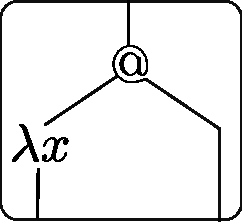
\includegraphics[scale=1.2]{pictures/redex.pdf}
\end{center}
that is, an application node whose left child is an abstraction node. In a well-typed $\lambda$-term, we define the \emph{type of a redex} to be the type of the left sub-term of its application node. In the figure above, the type of the redex is $\tau\rightarrow\sigma$. If the abstraction node of a redex is labeled by $\lambda x$, we say that $x$ is the variable of the redex and that it is an \emph{$x$-redex}. 

Let us go back to the proof of Thm.~\ref{prop:one-register}. We proceed by induction on the set of types $S$. The main observation is that, if the evaluation of a redex of type $\sigma\rightarrow \tau$ creates new redexes, then their types are either $\sigma$ or $\tau$, they are in particular in $S\setminus\{\sigma\rightarrow\tau\}$. Thus, we only need to show that the function that evaluates all the redexes of a fixed type is derivable. As we only create strictly smaller redexes, we need to iterate this process only finitely many times, the bound being the size of $S$. 

  Since we have only finitely many typed variables, it is enough to show that the function that evaluates all the redexes of a fixed type $\sigma$ and a fixed variable $x$ is derivable. This will be our goal in the rest of this section.

\begin{proposition}\label{thm:evalOneType}
 For every typed set $X$, every finite set $S$ of simple types and every $x\in X$ and $\sigma\in S$, the function 
    \begin{align*}
        M \in  \LinTerms S X \quad \mapsto \quad  \begin{array}{l}
        \text{The \lambdaterm obtained by reducing all}\\ \text{the $x$-redexes of type $\sigma$ in $M$} 
        \end{array}
    \end{align*}
    is derivable.
\end{proposition}

To show this proposition, we will factorize (via a derivable function) our \lambdaterms into factors satisfying the following properties:
\begin{itemize}
\item All the $x$-redexes of type $\sigma$ fall entirely into one of the factors. In other words, for every such redex, its application node, its abstraction node, and the variable it binds are in the same factor.
\item Each factor have a a very specific shape called \emph{thin}. Those factors, which are \lambdaterms with ports, are roughly speaking those terms whose normal form have the shape of a word (by opposition to trees, which is the general case).
\end{itemize}
Since each redex is fully contained in a thin factor, it is enough to show that normalization of thin \lambdaterms (with ports) is derivable. To do so, we prove that the word obtained by normalizing a thin \lambdaterm results from a depth-first traversal of the later. Using the fact that depth-first traversal is a basic function, we show that normalization of thin $\lambda$-terms is derivable.
 
 The last ingredient to conclude the proof is to notice that $\beta$-reducing the factors of (a factorization of) a $\lambda$-term, then applying a flattening, is the same thing as $\beta$-reducing the original $\lambda$-term, which is a direct consequence from the fact that $\beta$-reduction is a congruence on terms. This concludes the proof. 
 
 In the rest of this section, we develop on each of the two main steps of the proof.  In Sec.~\ref{subsub:thin} we present thin \lambdaterms with ports and show how to normalize them. Then we show in Sec.~\ref{subsub:facto} how to factorize a \lambdaterm into thin factors. 
 

\subsubsection{Evaluation of thin $\lambda$-terms}\label{subsub:thin}

As discussed earlier in the proof sketch, we will need to evaluate \lambdaterms with ports (the factors of our factorization). In the following, we will denote by $\lamrank X$ the ranked set 
\begin{align*}
     \overbrace{\set{x : x \in X}}^{\text{arity 0}} \cup \overbrace{\set{\lambda x : x \in X}}^{\text{arity 1}} \cup  \overbrace{\set @}^{\text{arity 2}}
\end{align*}
Thus, \lambdaterms with ports are the inhabitants of $\tmonad \lamrank X$. Normalization of these terms generalize that of usual \lambdaterms in a straightforward way: the $i$-th port is replaced by a fresh variable $x_i$, the obtained \lambdaterm (without ports) is evaluated as usual, then the variable $x_i$ is replaced back by the port $i$, as one can see in the following example.  
  \begin{center}
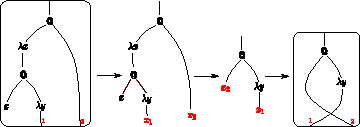
\includegraphics[scale=1.2]{pictures/normalization-with-ports.pdf}
\end{center}
  Note that when a \lambdaterm is linear, its normal form has the same number of ports. Note also that respecting the original order of ports in the normal form (which is important for compositionality) may twist ports, as in the example above. As a consequence, normalization of linear \lambdaterms with ports is an arity preserving function of  type:
  \begin{align*}
  \tmonad \lamrank X \to \reduce 1 \tmonad \lamrank X 
  \end{align*}
%Keeping the original order of ports in the normal form (which generates twists) is important for compositionality.
% Indeed, if the ports 1 and 2 of the left-most \lambdaterm of the example above was connected respectively to two terms $u$ and $v$, then its normal form would be 
   
Let us present now the class of \emph{thin \lambdaterms with ports}.
 
\begin{definition}
We say that the node of a $\lambda$-term is \emph{branching} if its has at two distinct children which are not ports.
 
A \emph{thin $\lambda$-term with ports} is a term from $\tmonad \lamrank X$ in which every branching node is the application node of a redex. In the remaining of this section we will omit the mention ``with ports'' if clear from the context.
%We denote by $\thinterm S X$ the set of thin $\lambda$-terms.
\end{definition}

Since thin $\lambda$-terms branch only on redexes, the result of their evaluation is a ``word'', in the sens that every node has at most one non-port child.  We will show that this word can actually be obtained by a depth-first traversal of the original $\lambda$-term. We will then use the basic depth-first traversal  function to show that normalization of thin $\lambda$-terms is derivable. 

The left $\lambda$-term below is linear and thin. The colored nodes are the ones which are not redexes nor the variables of these redexes. The right $\lambda$-term is its normal form: we can see that the order of in which the nodes appear top-down follows the depth-first traversal of the original $\lambda$-term.  
\begin{center}
		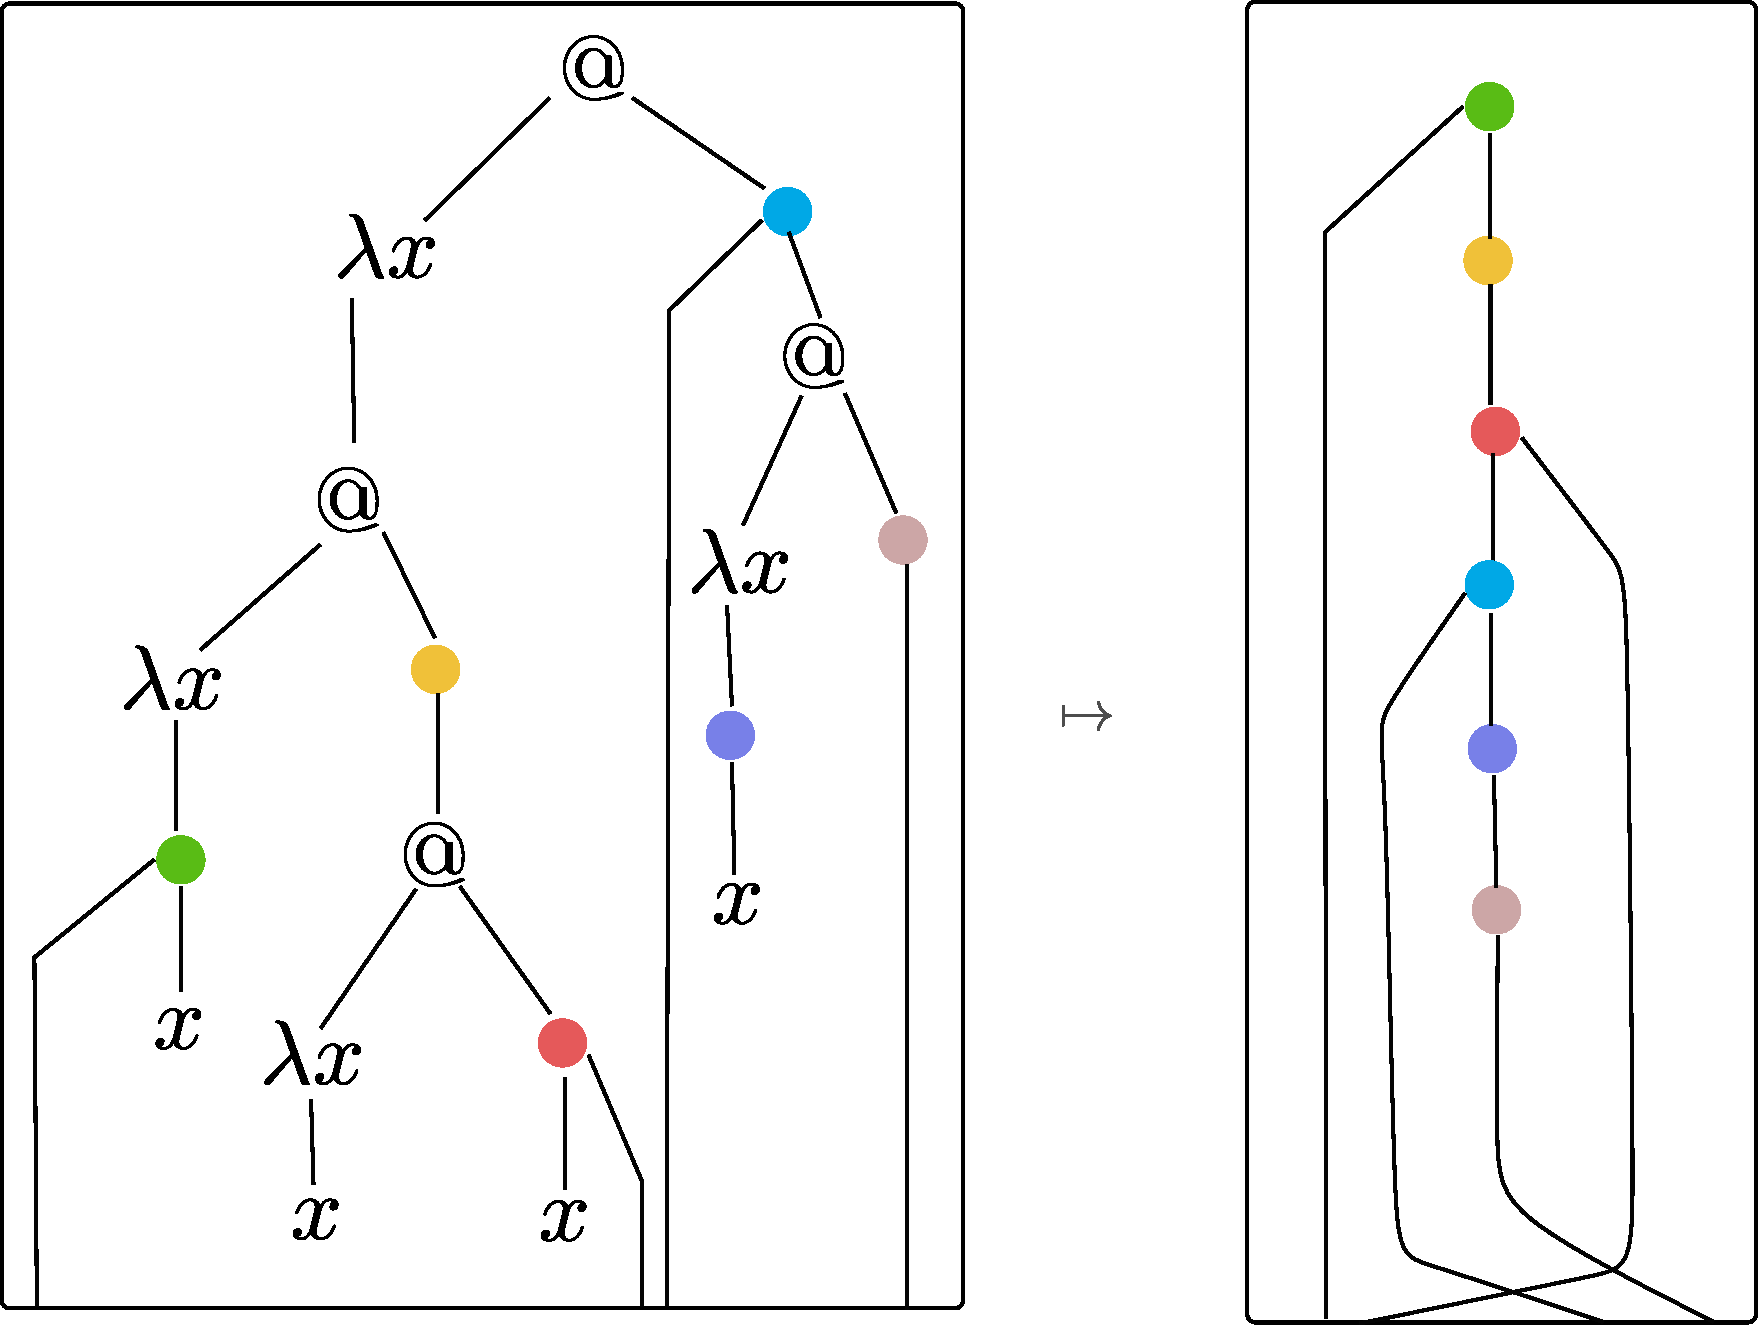
\includegraphics[scale=.2]{pictures/normalisation-thin}
		\end{center}

\begin{proposition}\label{prop:EvaluateThin}
 For every typed set $X$ and every finite set $S$ of simple types, the function 
    \begin{align*}
    \tmonad \lamrank X &\quad\to\quad \reduce 1 \tmonad \lamrank X\\
        M & \quad \mapsto \quad \text{normal form of $M$ if $M$ is linear and thin}
    \end{align*}
    is derivable.
\end{proposition}

Let $t$ be a strongly thin $\lambda$-term and let $u$ be its normal form. As noticed before, $u$ has the shape of a word. Moreover, since $t$ is linear, the nodes of $u$ are exactly the nodes of $t$ which are not redexes, nor their variables.

\begin{proposition}\label{prop:normal-form-depth-first} Let $t$ be a linear thin \lambdaterm and let $u$ be its normal form. 
The order in which the inner nodes (ie. non ports) of $u$ appear top-down is the depth-first order of $t$.  
\end{proposition}

\begin{proof}
To establish this proposition, we need the following lemma.
\begin{lemma}\label{lem:internalLemma}
Let $t$ be a linear thin $\lambda$-term and let $r$ be one of its redexes. Consider $m$ to be the binder node of $r$ and $n$ to be its variable node.

The node $n$ is the greatest (that is the left-most) node in the sub-term $t|_m$ w.r.t. the depth-first order. 
\end{lemma}

\begin{proof}
We proceed by induction on the length of the path between $m$ and $n$. When it is $0$ the result is clear. Suppose by contradiction that it is strictly greater than $0$ and that there is a node $o$ which is strictly greater than $n$. We take $o$ to be the smallest node which is greater than $n$. Since $t$ is thin, the least common ancestor $l$ between $n$ and $o$ is an application node of a redex. Since $n$ is smaller than $o$, $n$ is the left descendant  of $l$, in other words it is the descendant of the left child $p$
of $l$, which is a binder. The node $m, n, o$ and $p$ are illustrated below:
\begin{center}
		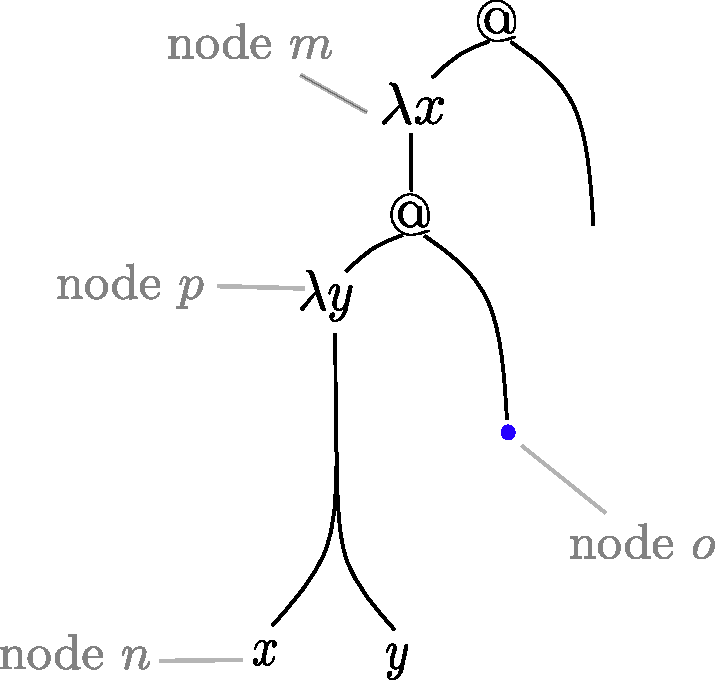
\includegraphics[scale=.3]{pictures/lemma-thin.pdf}
\end{center} 
 By induction hypothesis, the variable
bound by $p$ is strictly greater than $n$. Is is also strictly smaller than $o$, which gives a contradiction and concludes the proof. 
\end{proof}

Let us go back to the proof of our proposition. Consider two inner nodes $n, m$ of $t$ which are also nodes of $u$, and such that $m$ is smaller than $n$ is the tree order of $t$. We show that $n$ is a descendant of $m$ in $u$. There is two cases to consider:
\begin{itemize}
\item Either $n$ is a descendant of $m$ in $t$, in this case we can conclude easily since $\beta$-reduction preserves the descendant relation. Indeed, by a small analysis of $\beta$-reduction, one can notice that a reduction step may extend the descendant relation, but can never change (or break) the order of two comparable nodes in the original $\lambda$-term.  
\item  Otherwise, let us consider the lowest common ancestor $p$ of $m$ and $n$. We proceed by induction on the length of the path between $m$ and $p$. By definition of thin $\lambda$-terms, since $p$ is branching it is necessarily an application node, whose left child $q$ is a binder node, let us say $\lambda x$. 
By Lemma~\ref{lem:internalLemma}, $m$ is smaller w.r.t. the depth-first order than the node $r$ of the variable bound by $q$ . 
We are then left with the following two situations. The first case, illustrated by the left figure below, is when $r$ is a descendant of $m$ in $t$. In this case, after one reduction step $n$ will be a descendant of of $m$. The other case is when $m$ is in the left of $r$ in $t$, as illustrated by the right figure below. In this case, after one reduction step, the lowest common ancestor between $m$ and $n$ will be a descendant of $p$, and we can conclude by induction hypothesis. 
\begin{center}
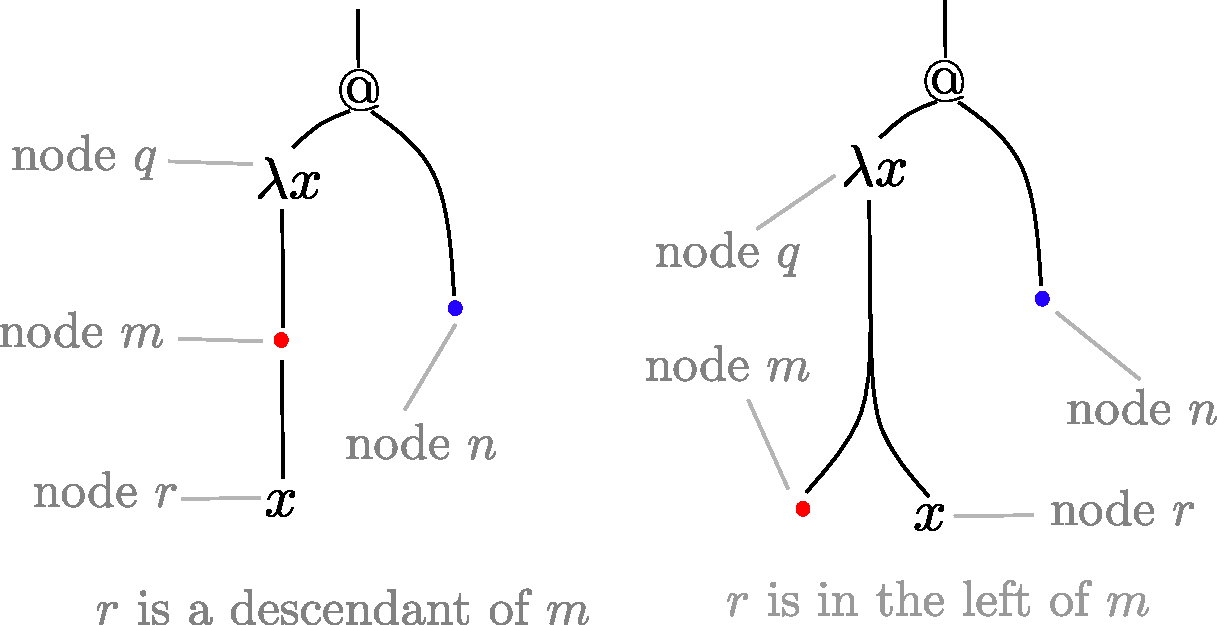
\includegraphics[scale=.3]{pictures/cases-lemma}
\end{center}
\end{itemize}
This concludes the proof of the first claim.
%\end{center}    
\end{proof}

Let us construct now a derivable function which computes the normal form of linear thin $\lambda$-terms. We illustrate this construction on the term $t$ below which will be our running example in this proof. 
\begin{center}
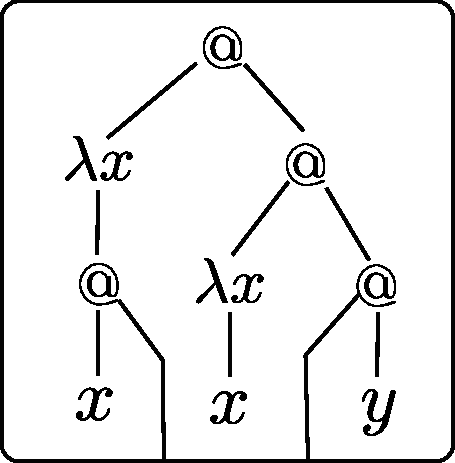
\includegraphics[scale=.3]{pictures/running-thin}
\end{center}

\begin{proof}[Proof of Proposition~\ref{prop:EvaluateThin}] Let $t$ be a linear thin $\lambda$-term in $\tmonad \lamrank X$.
%Let us show that the evaluation of thin $\lambda$-terms is derivable. We will consider an additional hypothesis on thin $\lambda$-terms:
%\begin{center}
%\textit{If a node is an application node of a redex, then it is branching.}$\qquad\qquad (H)$
%\end{center}
%Hypothesis $(H)$ is the converse of the condition on thin $\lambda$-terms. We will first show that normalization of thin $\lambda$-terms with this additional condition (let us call them strongly thin $\lambda$-terms) is derivable, then we will show later how to get rid of it.



%To establish the second claim, it is enough to show it for one step of $\beta$-reduction. But this last point is clear by a simple analysis of $\beta$-reduction, as far as we consider that the right child of the $@$ node of every redex is not a port. This is is guaranteed by the condition $(H)$ of strongly thin $\lambda$-terms. 

\begin{enumerate}
\item
We start by distinguishing the redexes of $t$ and their variables from the other nodes. For that, we apply the characteristic function of the following first-order query $\varphi$:
    \begin{center}
    ``The node $u$ is a redex or a variable of a redex''
    \end{center}
    This query is first-order expressible. Indeed it is the disjunction of the following queries
$$\begin{array}{rl}
@\mathsf{Redex}(u) = & @(u) \wedge \exists v \ \mathrm{Child}_1(u,v) \wedge \bigvee_{x\in X}\lambda x(v)\\[8pt]
\lambda\mathsf{Redex}(u)=& \lambda x(u) \wedge \exists v \ \mathrm{Child}_1(v,u) \wedge @(v) \\[8pt]
X\mathsf{Redex}(u) = &\bigvee_{x\in X} x(u) \wedge \exists v\ \lambda\mathsf{Redex}(v) \wedge v\ \mathsf{binds}\ u
\end{array}$$
where $@\mathsf{Redex}(u)$ says that $u$ is the application node of a redex, $\lambda\mathsf{Redex}(u)$ says that it is the abstraction node of a redex and $X\mathsf{Redex}(u)$ says that it is the variable of a redex. 
The formula $u\ \mathsf{binds}\ v$, defined below,  is a binary first-order query expressing that the node $u$ is an abstraction node that binds $v$.
 \begin{align*}
 \bigvee_{x\in X} \lambda x(u) \wedge x(v) \wedge u<v\wedge \forall u<w<v\ \neg \lambda x(w)
 \end{align*}

The query $\varphi$ being first-order, its characteristic function is derivable thanks to Proposition~\ref{prop:forat}. 

When we apply this function to $t$, we get a term in $\tmonad(\lamrank X+\lamrank X)$ term below. 
Below is the effect of this first step on our running example. We colored in red the nodes belonging to the first copy of $\lamrank X$, that is the nodes satisfying the query $\varphi$. These nodes are the ones that will disappear in the normal form of $t$. 
\begin{center}
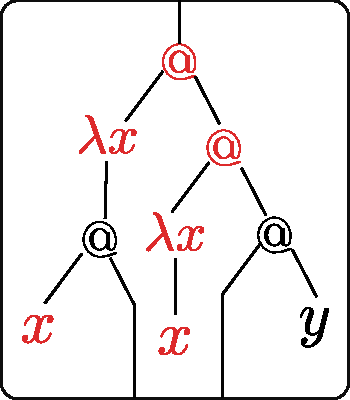
\includegraphics[scale=.3]{pictures/running-thin-2}
\end{center}
\item After that, we apply the depth-first traversal function 
\begin{align*}
            \ranked{\preorder : \tmonad (\lamrank X+\lamrank X) \to \reduce 1\tmonad( \lamrank X+\lamrank X + 0 +2)}
\end{align*}
After this step, our initial term becomes
\begin{center}
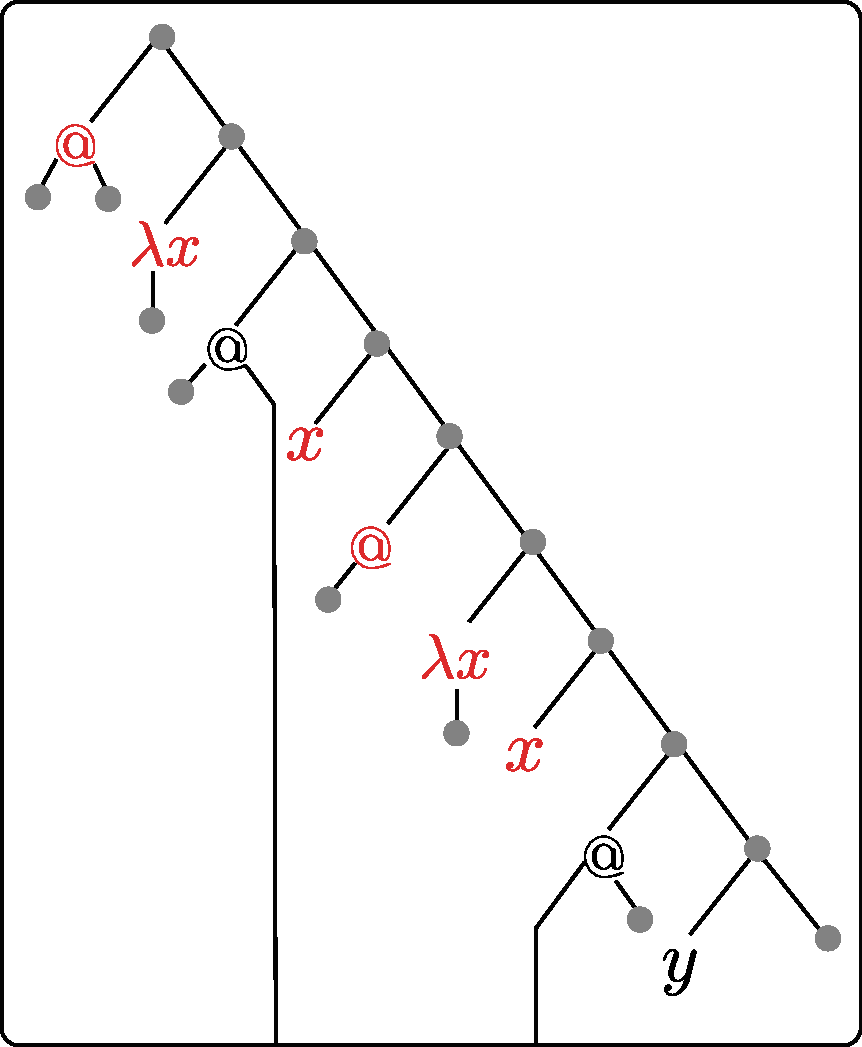
\includegraphics[scale=.3]{pictures/running-thin-3}
\end{center}  
In this term, the nodes of the normal form appear in the right order thanks to Prop.~\ref{prop:normal-form-depth-first}. Now, we only need to get rid of the redexes and the variable nodes that participated in the computation of the normal form (that is the ones colored in red) together with the nodes $\grayball$ and $\grayballbin$ introduced by the depth-first traversal function. 
\item For this purpose, we apply the function 
\begin{align*}
\ranked{\mathsf{Tagg}}: \ranked{\tmonad (X^\lambda+X^\lambda + 0+
2)} \to \ranked{\tmonad (X^\lambda+X^\lambda + 0+2+1) }
\end{align*}
 which adds the unary symbol $1$ as the parent of every node $2$. This function can be easily implemented using the derivable homomorphism function of Example~\ref{ex:morphism}. Then we apply the factorization $\ancfact$
 to separate the symbol $1$ from the others:
 \begin{align*}
 \ranked{\ancfact : \tmonad (X^\lambda+X^\lambda + 0+2+1) \to \tmonad (\tmonad(X^\lambda+X^\lambda + 0+2)+\tmonad 1))}
 \end{align*}
 
 After this step, our example term becomes    
\begin{center}
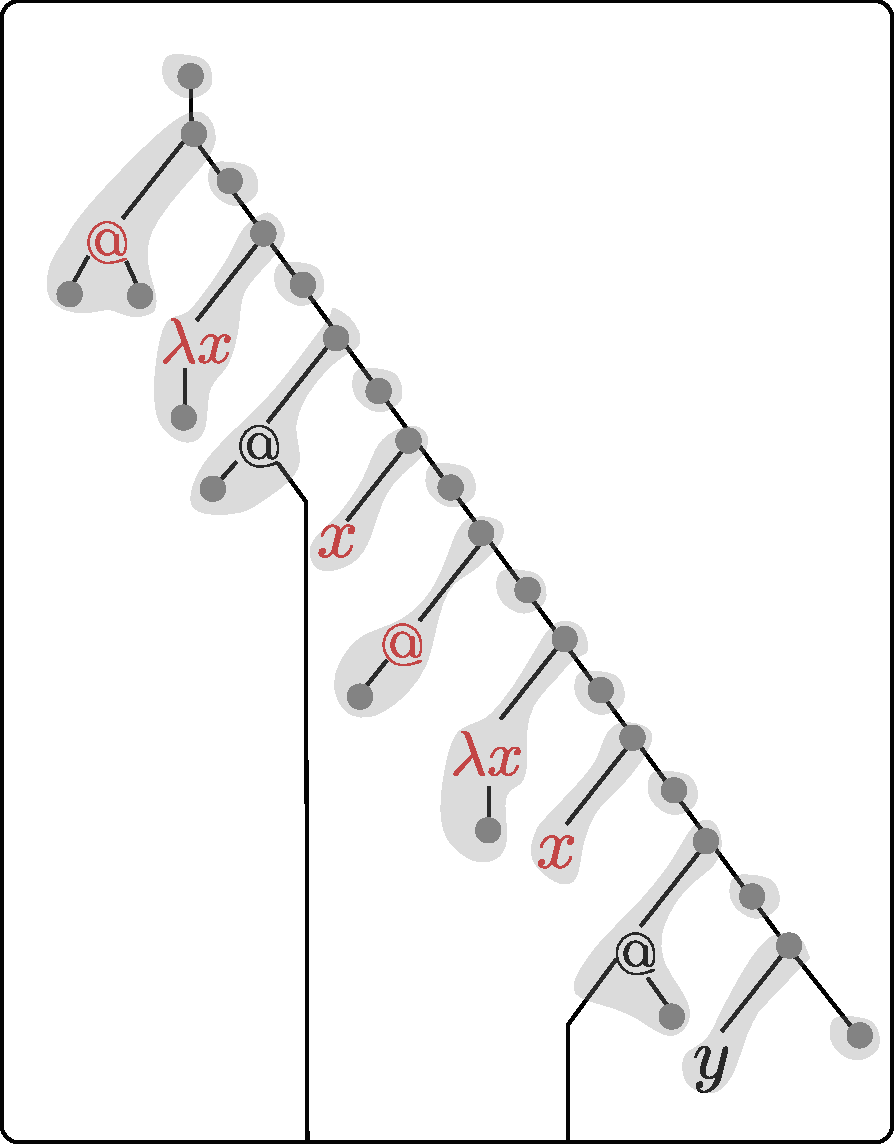
\includegraphics[scale=.3]{pictures/running-thin-4}
\end{center}

\item Now consider the function 
 \begin{align*}
 \ranked{g: \tmonad(X^\lambda+X^\lambda+0+2) \to \reduce 1\tmonad(X^\lambda+X^\lambda+0+2)}
 \end{align*}
 which is the identity function, except for the following finite set of terms for which it is defined in figure~\ref{fig:definition-g}.
\begin{figure*}
\begin{center}
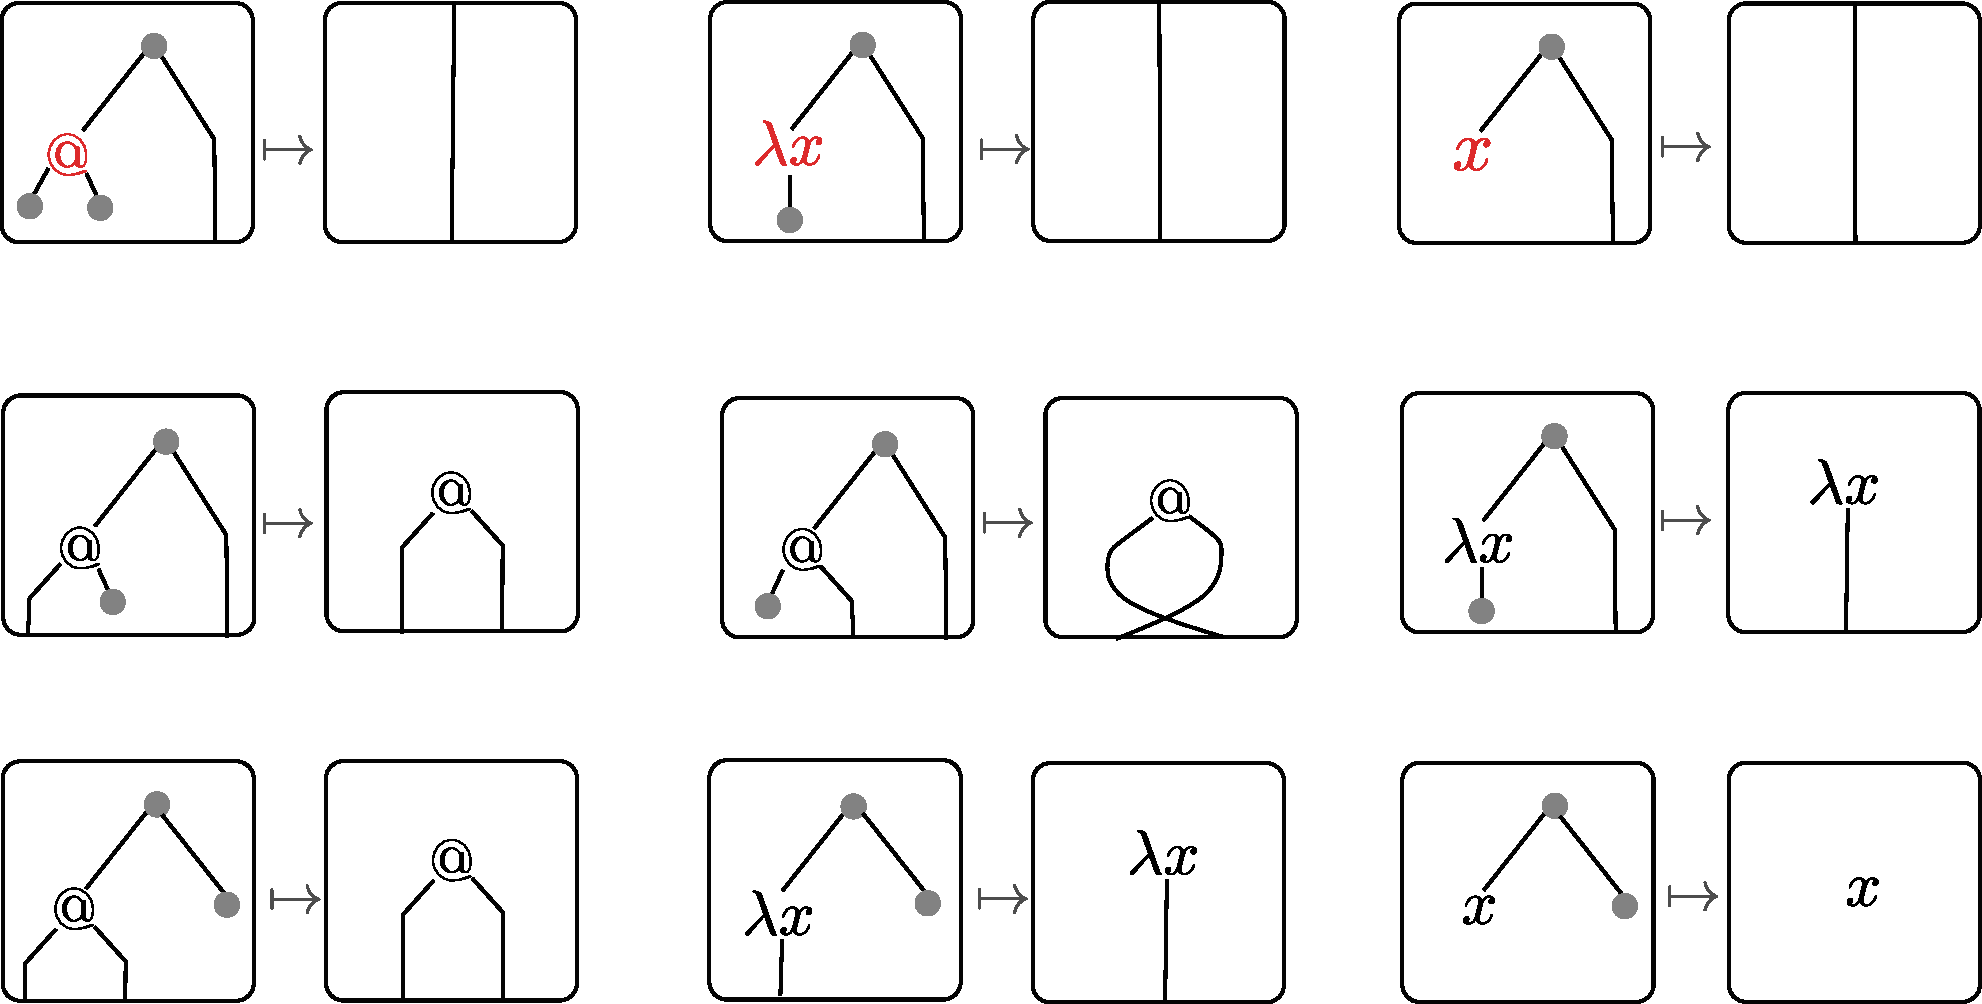
\includegraphics[scale=.3]{pictures/function-g}
\end{center}
\caption{Definition of the function $g$.} \label{fig:definition-g}
\end{figure*}
The red elements are those belonging to the first copy of $\lamrank X$.
\smallskip

Now back to our term, we replace the  $\ranked{\tmonad 1}$ factors by the empty term, and to the other factors we apply the function $g$. After that, we apply the function 
\begin{align*}
\ranked{\reduce 1\reduce 1 \Sigma \to \reduce 1\Sigma}
\end{align*}
which untwists two consecutive applications of $\reduce 1$. Doing so, we get a term of type  $$\ranked{\reduce 1\tmonad(X^\lambda+X^\lambda+0+2)}$$ which is  the normal form of $t$. Our running example becomes then
\begin{center}
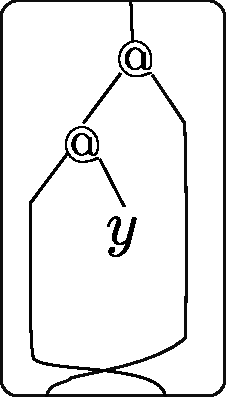
\includegraphics[scale=.3]{pictures/running-thin-5}
\end{center}

\item Note that we obtained the desired term, but not with the desired type. To obtain a term in 
$\ranked{\reduce 1\tmonad{X^\lambda}}$, we get rid of the labels $0+2$ by transforming them respectively into variables and application nodes. The choice of which variables to choose is not important, since the only terms that will actually have $0+2$ in their results are \lambdaterms which are not linear or not thin.
\end{enumerate}
\end{proof}

  



\subsubsection{Factorizing $\lambda$-terms into blocks of thin $\lambda$-terms}\label{subsub:facto}

In a linear $\lambda$-term, we call \emph{full redex} a set of nodes  containing a redex, the node of its variable, together with the set of nodes between them, as illustrated below
\begin{center}
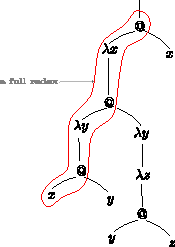
\includegraphics[scale=1.2]{pictures/full-redex.pdf}
\end{center}


\begin{proposition}\label{prop:FactoIntoThin} For every finite set of typed variables $X$, for every finite set of types $S$ and for every $x\in X$ and $\sigma\in S$, there is a factorization $$\ranked{f:\tmonad \ranked{X^\lambda} \to \tmonad\tmonad \ranked{X^\lambda}}$$ 
such that for every linear \lambdaterm $t$
\begin{itemize}
\item every full $x$-redex of type $\sigma$ in $t$ is entirely contained in one of the factors of $f(t)$;
\item the factors of $f(t)$ are thin.
\end{itemize}
\end{proposition}

\begin{proof}
We define the function $f$ as the composition of the following three functions
\begin{align*}
\ranked{\tmonad \ranked{X^\lambda} \xrightarrow{\ g\ } \tmonad (\ranked{X^\lambda}+1) \xrightarrow{\ \mathsf{block}^\uparrow\ } \tmonad (\tmonad\ranked{X^\lambda}+\tmonad 1)
\xrightarrow{\ \mathsf{erase}\ } \tmonad \tmonad\ranked{X^\lambda}}
\end{align*}
The function $g$ is a first-order rational tree function, which indicates, using the unary symbol $1$, the places wheres two distinct blocks of $f$ will be separated. We will describe it more precisely a bit later. The function $\mathsf{block}^\uparrow$ will create these blocks and finally, we erase all the factors $\ranked{\tmonad 1}$.

The functions $\mathsf{block}^\uparrow$ is a basic function and  $\mathsf{erase}$ can be easily derivable. 
Let us show how to derive the function $g$, so that the $1$-nodes it introduces creates blocks satisfying the conditions 1 and 2 of Proposition~\ref{prop:FactoIntoThin} (when the input is a linear $\lambda$-term).  

We define $g$ as the composition of the characteristic function of three first-order unary queries: $\mathsf{@redex}, \mathsf{Right}$ and $\mathsf{Left}$, followed by a homomorphims $h$. We define them in the following:
\begin{itemize}
\item The property $\mathsf{@Redex}$ checks whether a node is the application node of an $x$-redex of type $\sigma$. It can be expressed by the following first-order formula, where  $\varphi_\sigma$ is a first-order formula which decides if the type of a node is $\sigma$ (for instance the one given by Lemma~\ref{lem:IsTypeTauFo}):
\begin{align*} \mathsf{App}( u ):=& \mathsf{@}(u)\ \wedge\ \exists v\  \mathrm{Succ}_1(u, v) \wedge \lambda x(v)\ \wedge\ \varphi_\sigma(v)
\end{align*} 
\item The query $\mathsf{Right}$ (resp. $\mathsf{Left}$) checks if the node is an application node, which lies, together with his right (resp. left) child, between the application node of an $x$-redex of type $\sigma$ and the node it binds. Those properties can be easily expressed by a first-order formula.
\end{itemize}

When we apply the characteristic functions of these queries to a term in $\ranked{\tmonad X^\lambda}$, each node will be decorated by three informations: whether is satisfies or not $\mathsf{App}$,  whether is satisfies or not $\mathsf{Right}$ and whether is satisfies or not $\mathsf{Left}$. Note that for linear $\lambda$-terms, some combinations of these properties cannot hold in the same node. For instance, a node cannot satisfy $\mathsf{Right}$ and $\mathsf{Left}$ simultaneously, as this would contradict linearity. 

Now we define the homomorphism $h$, which maps the $\lambda$-terms with these three informations to terms of $\ranked{\tmonad (\ranked{X^\lambda}+1)}$. We define the action of $h$ on each node, depending on its label and the three informations it contains:
\begin{itemize}
\item If the label of the node is $y$ or $\lambda y$ for some variable $y\in X$, or if the label is $@$ and satisfies $\mathsf{App}$, then $h$ returns the same node (seen as a term), forgetting the extra three informations.
\item If the node is an application node satisfying 
\begin{align*}
\neg \mathsf{App} \wedge \neg \mathsf{Right} \wedge\neg \mathsf{Left} 
\end{align*} 
then $h$ adds $1$ to the two children of the node.
\item If the node is an application node satisfying 
\begin{align*}
\neg \mathsf{App} \wedge \neg \mathsf{Right} \qquad\text{(resp. } \neg \mathsf{App} \wedge \neg \mathsf{Left} \text{)}
\end{align*} 
then $h$ adds $1$ to the left (resp. right) child of the node. 
\end{itemize}
Let $t$ be a linear $\lambda$-term. We show that the factors induced by $g$ satisfy the two conditions of Proposition~\ref{prop:FactoIntoThin}. First of all, by analyzing the action of $h$ on each node, note that every application node will receive $1$ as one of its children, except when it is satisfies $\mathsf{App}$. Thus the only branching nodes in a factor are redexes, hence the factors are thin. Now suppose by contradiction that there is some full $x$-redex of type $\sigma$ of $t$ which is not entirely contained in a factor. This means that in $g(t)$ there is a $1$ between the application node of some $x$-redex of type $\sigma$ and its variable.
By construction of $h$, $1$ is the child of an application node (call it $n$). Suppose w.l.o.g. that it is the right child of $n$. The node $n$ cannot satisfy $\mathsf{App}$ because it got $1$ as a child by $h$. Is satisfies $\mathsf{Right}$ by the contradiction hypothesis. Thus its satisfies $\neg \mathsf{App} \wedge \neg \mathsf{Right}$, therefore it receives also $1$ as its left child by $h$. This means that $n$ received $1$ for its both children, and the only way to get that is to satisfy $\neg \mathsf{App} \wedge \neg \mathsf{Right} \wedge\neg \mathsf{Left}$, which gives a contradiction. 
\end{proof}
%\subsubsection{$\beta$-reduction commutes with factorization} \label{subsub:commutes}
%The last ingredient to show Thm.~\ref{thm:evalOneType} is to notice  that factorizing a term, applying some $\beta$-reduction steps to the factors, then flattening, can be simulated by applying  $\beta$-reduction steps directly to the original $\lambda$-term.
%
%Let us state this property more formally. For that, we can generalize the lifting of functions to the lifting of relations as follows. 
%Let $\Sigma$ be a ranked set. If $R\subseteq \ranked{\Sigma}\times\ranked{\Sigma}$ is an arity preserving relation (that is $\arity{u}=\arity{v}$ whenever $(u,v)\in R$), then $R$ can be lifted to $\tmonad R\subseteq \ranked{\tmonad \Sigma} \times \ranked{\tmonad \Sigma}$ in a natural way. 
%
%Since $\beta$-reduction is an arity preserving relation  over linear $\lambda$-terms, its reflexive transitive closure $\beta^*$ is arity preserving as well.  We can lift then the later to $\tmonad \beta^*\subseteq \linterm S X\times\linterm S X$.
%The following proposition is a direct consequence from the fact that $\beta$ is a congruence on terms.
%
%\begin{proposition}\label{prop:betaCommutesWithFacto}
%For every factorization $f:\linterm S X \to \linterm S X$ and every linear $\lambda$-term $M$
%$$\text{if }\qquad f(M) \xrightarrow{\tmonad \beta^*} N \qquad\text{ then }\qquad M\xrightarrow{\beta^*} \flatt(N).$$
%\end{proposition}
%
%
